\section{Tuning}

Your Ukulele needs to be in tune. This means that each string has a certain pitch. Even though this is already implied, it is important to note that the relative pitch different per string is important as well. In \autoref{fig:ukulele_string_names} you see the names (letters) of the string.

\begin{figure}[h]
    \centering
    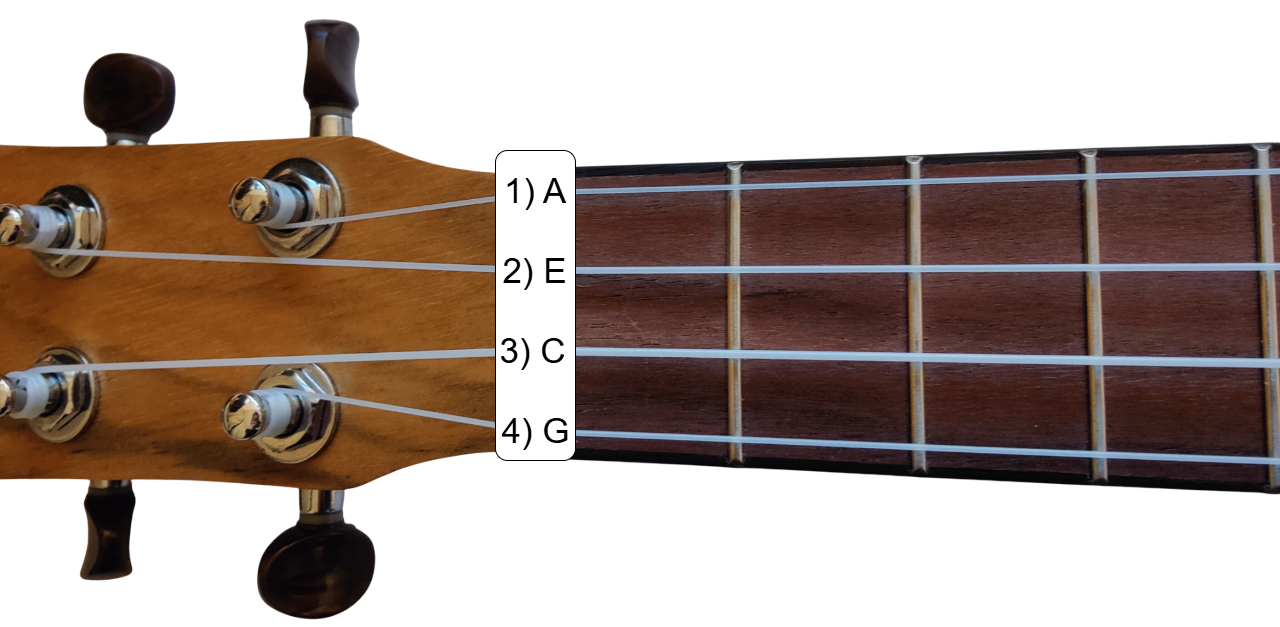
\includegraphics[width=0.42\textwidth]{../../Images/UkuleleNeck-StringNames.png}
    \caption{Names of the ukulele strings}
    \label{fig:ukulele_string_names}
\end{figure}

A mnemonic is (from string 4 to 1):

\begin{itemize}
	\setlength\itemsep{0em}
	\item[4)] \textbf{G} ood
	\item[3)] \textbf{C} cooks
	\item[2)] \textbf{E} eat
	\item[1)] \textbf{A} all 
\end{itemize}


\begin{minipage}{0.5\textwidth}
You use a tuner to tune (see \autoref{fig:ukulele-tuning}). The tuner either gives a note value, and then you have to tune up or down to get the correct note on the screen. Or it shows a string number and you have to get the 'pointer' in the middle.

Be careful with tuning the string up (to a higher pitch). Especially the thinner strings can break if they are too right.
\end{minipage}
\hfill
\begin{minipage}{0.3\textwidth}
	\centering
	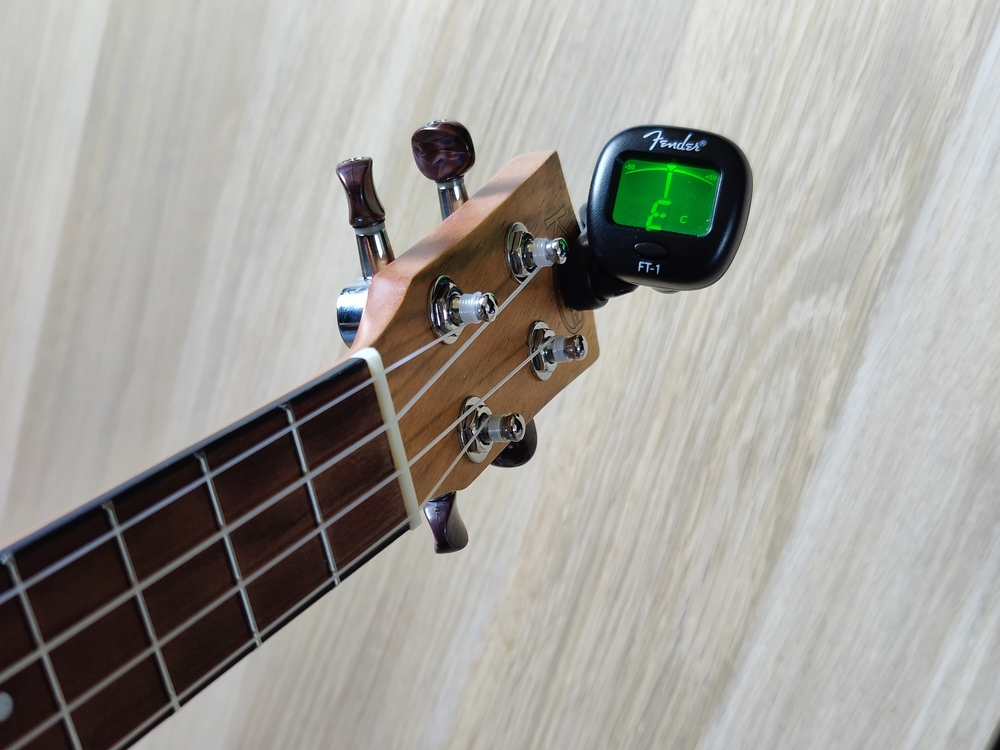
\includegraphics[width=\textwidth]{../../Images/ukulele-tuning.jpg}
	\captionof{figure}{Using a tuner on a ukulele}
	\label{fig:ukulele-tuning}
\end{minipage}

Another tuning options relies on the previously mentioned difference in pitch between the strings. In \autoref{fig:ukulele_relative_tuning} you see which positions on the neck have the same pitch the a thinner open string.

\begin{figure}[h]
	\centering
	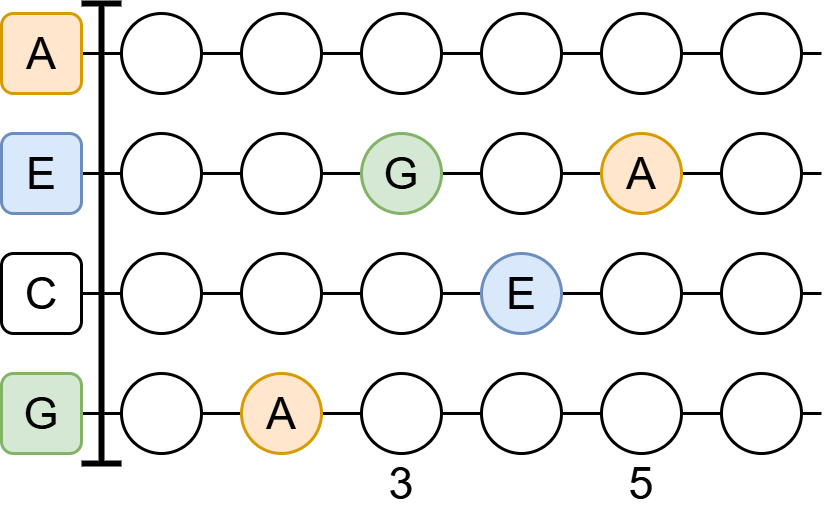
\includegraphics[width=0.38\textwidth]{../../Images/UkuleleRelativeTuning.png}
	\caption{Relative tuning}
	\label{fig:ukulele_relative_tuning}
\end{figure}
